\section{Applying RISE}
Problem: returned classes from RISE do not match with precalculated classes
=> normalize was not applied on find\_best\_images.
=> use same function on all image loaders

\nblink{nhs-chest-xray/analyze/rise.ipynb}
\nblink{nhs-chest-xray/analyze/rise\_bounding\_boxes.ipynb}

\subsection{Results}
\begin{figure}[H]
\centering
\caption{RISE example 1}
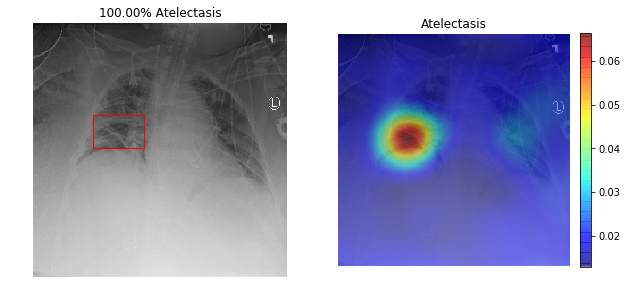
\includegraphics[width=12cm]{chapters/03_classification/images/rise_0.png}
\end{figure}

\begin{figure}[H]
\centering
\caption{RISE example 2}
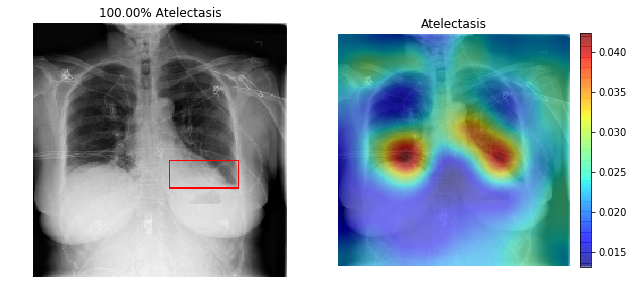
\includegraphics[width=12cm]{chapters/03_classification/images/rise_2.png}
\end{figure}

\begin{figure}[H]
\centering
\caption{RISE example 3}
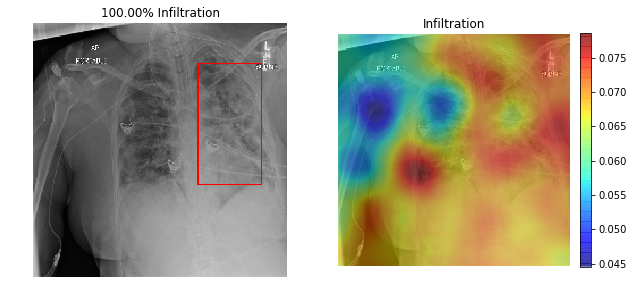
\includegraphics[width=12cm]{chapters/03_classification/images/rise_8.png}
\end{figure}

\subsection{Discussion}
Looks good for most, some (like the last image) are very bad.
